\documentclass{article}
\usepackage{graphicx} % Required for inserting images

\title{\Large{\textbf{Exercise 3: BFS, DFS, and A* Comparison}}}
\author{Roxanne Ysabel Resuello}
\date{September 2023}

\begin{document}

\maketitle

% INTRODUCTION
\section{Performance of breadth-first search (BFS), depth-first search (DFS), and A* for solving the 8-puzzle Game}

The performance of BFS, DFS, and A* differs in terms of time and space complexity which is evident through the number of paths explored. Thus, there are times when these algorithms result in different solutions or paths. For BFS, it first explores all the states at the next level before going deep into a certain path or branch. Space complexity may be huge for this one since it needs to store all possible moves in the current state. Its time complexity would depend on how deep the goal is. If the goal puzzle is deep within a path, it will take a long time to find the solution. However, BFS guarantees an optimal solution since it explores all possible states at a level. This is evident in test case 1 in the table below. BFS and A* found the same optimal path, however, BFS explored more states which caused more time and space compared to A* algorithm.\\\\
DFS differs from BFS in terms of how it traverses the puzzle where it goes down deep through a path. Space complexity for this would depend on the depth of the goal, but unlike BFS where it stores all the states at all level, DFS only needs to store the current path from the initial puzzle. In this problem, DFS mostly takes a longer time than BFS since the path here is not limited. There are times that it may loop through or go too deep to a specific path before arriving at the goal puzzle.\\\\
Among the three algorithms, A* has a more efficient way of solving in terms of time and space complexity, while also arriving at the best path. Since this algorithm uses a heuristic function, it prioritizes exploring the puzzle with the least path cost. Thus, this avoids spending time and space exploring states that are far from the goal state.


\subsection{Among the three, which is the most appropriate approach for solving the 8-puzzle game? Which is the least appropriate approach?}

The most appropriate approach for solving the 8-puzzle game is the A* algorithm since it guarantees an optimal solution. As seen in test case 1, BFS and A* arrived at the same path, however, A* explored fewer states than BFS. This is brought by the heuristic function that significantly reduces the number of states to be explored. On the other hand, DFS is the least appropriate approach for this puzzle due to the unlimited depth of a path. This can also be seen in the table below where this explores a significantly higher number of states than BFS and A*. Apart from that, this also doesn't guarantee an optimal solution even though there are times that its time complexity of DFS is faster than other algorithms.


\section{Differentiate informed from uninformed search strategies.}

The behavior of informed and uninformed searches differ in picking which state to explore. Due to the heuristic function, informed search like A* algorithm prioritizes a state with a lesser heuristic value. On the contrary, an uninformed search like BFS or DFS chooses a current state based only on the sequence it was added on the frontier. This does not consider which state is nearest to the goal. Their difference in behavior results in different performances as well. Informed search has a more efficient performance since the heuristic function minimizes the number of explored states. An uninformed search explores many states that may not lead to a solution, thus, more time and space are generally used.

\begin{figure}
\centering
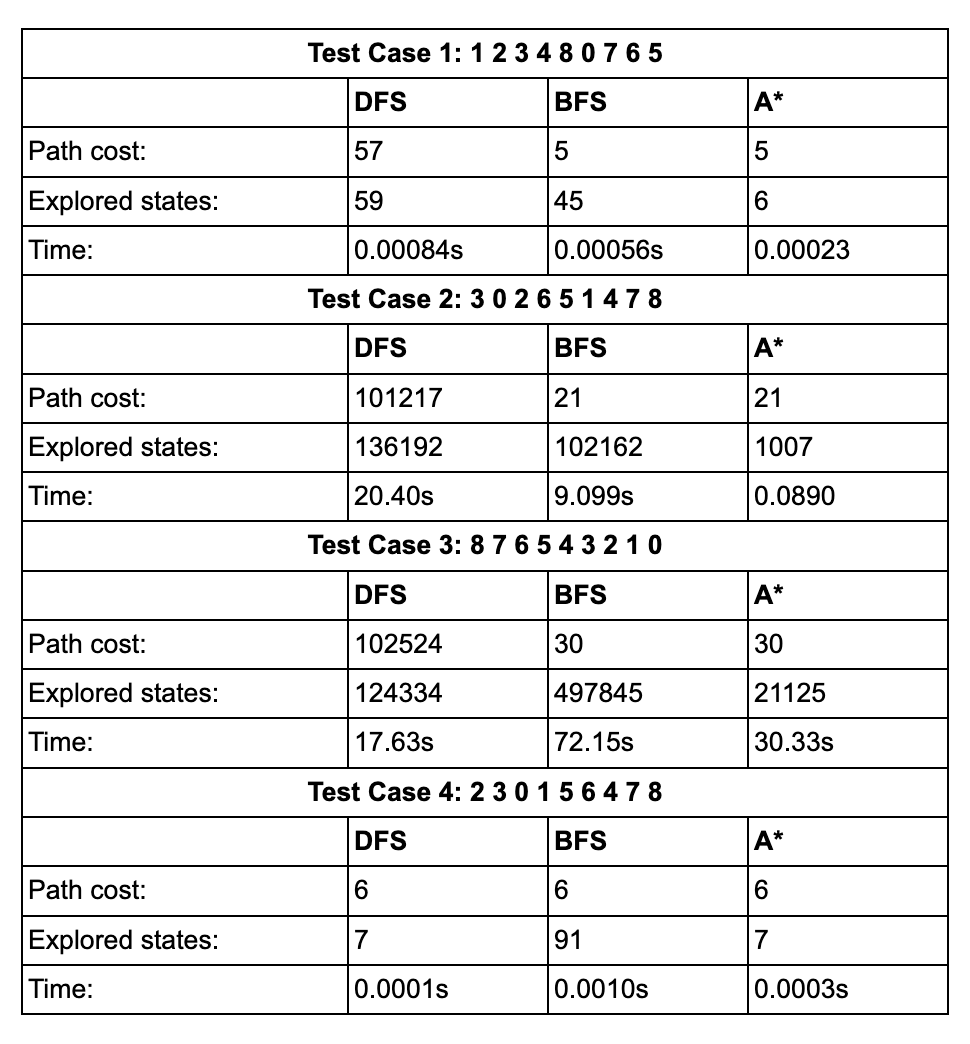
\includegraphics[width=\linewidth]{table.png}
\caption{\label{fig:table}Test Cases table.}
\end{figure}


\end{document}